\documentclass[../besoin_sys.tex]{subfiles}
\begin{document}
\section{Lobby}

Au lancement d'une partie, l'interface du lobby est affiché. On peut à ce moment inviter de nouveaux joueurs. 
Le lobby est joignable par d'autres joueurs sans nécessairement avoir envoyé d'invitations.
Le système s'occupera de les ajouter au lobby et les définiras en tant que spectateur.
Il faudra alors en définir un en tant que second joueur. Une fois cela fait, on peut lancer la partie.
Le système s'occupera de vérifier cette contrainte et de passer au lancement de la game.

\begin{figure}[h]
    \centering
    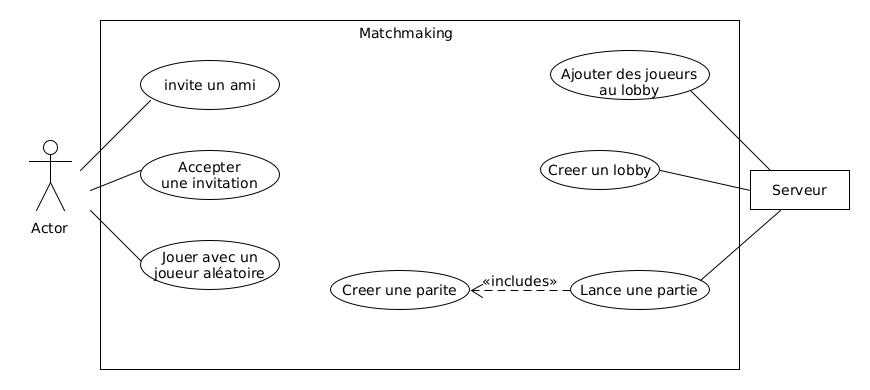
\includegraphics[scale=0.6]{img_fonctionnel/usecas_sys_matchmaking.png}
    \label{fig:Lobby}
    \caption{Lobby}
\end{figure}
\end{document}